\documentclass[11pt,a4paper]{article}

% Packages
\usepackage[utf8]{inputenc}
\usepackage[T1]{fontenc}
\usepackage{geometry}
\usepackage{amsmath,amssymb}
\usepackage{graphicx}
\usepackage{xcolor}
\usepackage{enumitem}
\usepackage{tcolorbox}
\usepackage{tikz}
\usepackage[hidelinks]{hyperref}
\usepackage{fancyhdr}
\usepackage{titlesec}
\usepackage{booktabs}
\usepackage{array}
\usepackage{listings}
\usepackage{multicol}
\usepackage{mdframed}

% Page geometry
\geometry{margin=0.9in}
\setlength{\headheight}{14pt}

% Colors
\definecolor{pytorchcolor}{RGB}{238,76,44}
\definecolor{conceptbg}{RGB}{240,248,255}
\definecolor{codebg}{RGB}{248,248,248}
\definecolor{importantbg}{RGB}{255,250,230}
\definecolor{tipbg}{RGB}{240,255,240}
\definecolor{warningbg}{RGB}{255,245,245}
\definecolor{codegreen}{RGB}{0,128,0}
\definecolor{codegray}{RGB}{128,128,128}
\definecolor{formulabg}{RGB}{245,245,255}

% Code listing style
\lstset{
    language=Python,
    basicstyle=\ttfamily\small,
    keywordstyle=\color{pytorchcolor}\bfseries,
    commentstyle=\color{codegray}\itshape,
    stringstyle=\color{codegreen},
    breaklines=true,
    frame=single,
    backgroundcolor=\color{codebg},
    showstringspaces=false,
    tabsize=4,
    morekeywords={torch,nn,optim,self,True,False,None}
}

% Custom boxes
\tcbuselibrary{skins,breakable}

\newtcolorbox{conceptbox}[1][]{
    colback=conceptbg,
    colframe=blue!60!black,
    fonttitle=\bfseries,
    title=#1,
    breakable
}

\newtcolorbox{importantbox}[1][Key Concept]{
    colback=importantbg,
    colframe=orange!70!black,
    fonttitle=\bfseries,
    title=#1,
    breakable
}

\newtcolorbox{tipbox}[1][Tip]{
    colback=tipbg,
    colframe=green!60!black,
    fonttitle=\bfseries,
    title=#1,
    breakable
}

\newtcolorbox{warningbox}[1][Warning]{
    colback=warningbg,
    colframe=red!60!black,
    fonttitle=\bfseries,
    title=#1,
    breakable
}

\newtcolorbox{formulabox}[1][Formula]{
    colback=formulabg,
    colframe=purple!60!black,
    fonttitle=\bfseries,
    title=#1,
    breakable
}

% Header/Footer
\pagestyle{fancy}
\fancyhf{}
\fancyhead[L]{\textcolor{pytorchcolor}{\textbf{Course 1: Deep Learning Fundamentals}}}
\fancyhead[R]{PyTorch Specialization}
\fancyfoot[C]{\thepage}

% Title formatting
\titleformat{\section}{\Large\bfseries\color{pytorchcolor}}{\thesection}{1em}{}
\titleformat{\subsection}{\large\bfseries\color{blue!70!black}}{\thesubsection}{1em}{}
\titleformat{\subsubsection}{\normalsize\bfseries\color{black!70}}{\thesubsubsection}{1em}{}

\begin{document}

% Title Page
\begin{titlepage}
    \centering
    \vspace*{1.5cm}
    
    {\Huge\bfseries\color{pytorchcolor} Course 1\\[0.3cm]}
    {\LARGE Deep Learning Fundamentals\\[1.5cm]}
    
    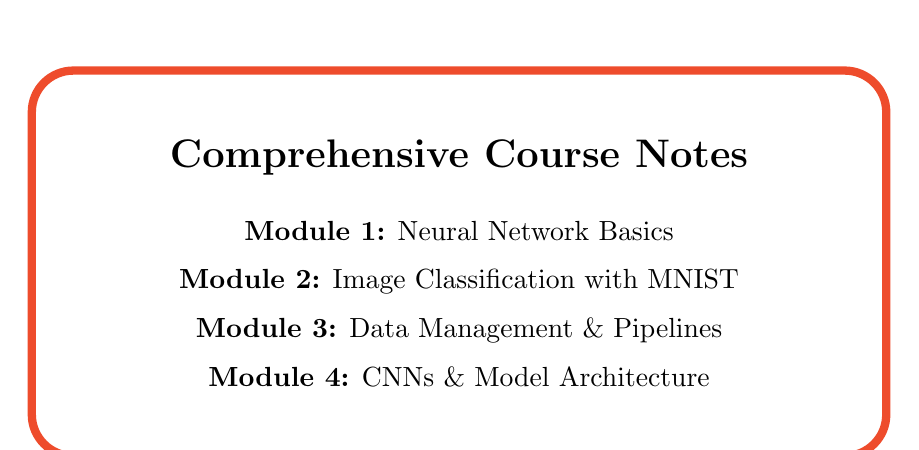
\begin{tikzpicture}
        \node[draw=pytorchcolor, line width=3pt, rounded corners=15pt, inner sep=25pt, fill=white] {
            \begin{minipage}{0.75\textwidth}
                \centering
                \Large\textbf{Comprehensive Course Notes}\\[0.5cm]
                \normalsize
                \textbf{Module 1:} Neural Network Basics\\[0.2cm]
                \textbf{Module 2:} Image Classification with MNIST\\[0.2cm]
                \textbf{Module 3:} Data Management \& Pipelines\\[0.2cm]
                \textbf{Module 4:} CNNs \& Model Architecture
            \end{minipage}
        };
    \end{tikzpicture}
    
    \vfill
    
    \begin{tikzpicture}
        \draw[pytorchcolor, line width=2pt] (0,0) -- (12,0);
    \end{tikzpicture}
    
    \vspace{1cm}
    {\large PyTorch Deep Learning Specialization}\\[0.5cm]
    {\large\today}
\end{titlepage}

% Table of Contents
\tableofcontents
\newpage

%==============================================================================
% MODULE 1: NEURAL NETWORK BASICS
%==============================================================================
\section{Module 1: Neural Network Basics}

\subsection{Introduction to Neural Networks}

Neural networks are computational models inspired by biological neurons. At their core, they learn patterns from data to make predictions.

\begin{importantbox}[The Machine Learning Pipeline]
\begin{enumerate}
    \item \textbf{Data Ingestion:} Gathering raw data from sources
    \item \textbf{Data Preparation:} Cleaning, normalizing, and formatting
    \item \textbf{Model Building:} Defining the architecture
    \item \textbf{Training:} Learning patterns from data
    \item \textbf{Evaluation:} Testing on unseen data
    \item \textbf{Deployment:} Using the model in production
\end{enumerate}
\end{importantbox}

\subsection{The Single Neuron Model}

A single neuron implements a simple linear equation:

\begin{formulabox}[Linear Equation]
$$\text{Output} = W \times \text{Input} + B$$

Where:
\begin{itemize}
    \item $W$ = Weight (slope of the line)
    \item $B$ = Bias (y-intercept)
\end{itemize}
\end{formulabox}

\begin{lstlisting}[caption=Creating a Simple Linear Model]
import torch
import torch.nn as nn

# Single neuron: 1 input -> 1 output
model = nn.Sequential(nn.Linear(1, 1))

# Access learned parameters
layer = model[0]
weight = layer.weight.data  # W
bias = layer.bias.data      # B
\end{lstlisting}

\subsection{Tensors: The Foundation of PyTorch}

\begin{conceptbox}[What are Tensors?]
Tensors are multi-dimensional arrays optimized for:
\begin{itemize}
    \item \textbf{GPU acceleration} - Fast parallel computation
    \item \textbf{Automatic differentiation} - Computing gradients automatically
    \item \textbf{Broadcasting} - Operations between different shapes
\end{itemize}
\end{conceptbox}

\subsubsection{Creating Tensors}

\begin{lstlisting}[caption=Tensor Creation Methods]
import torch
import numpy as np

# From Python lists
x = torch.tensor([1, 2, 3])
x = torch.tensor([[1.0], [2.0], [3.0]], dtype=torch.float32)

# From NumPy arrays
numpy_arr = np.array([1, 2, 3])
tensor = torch.from_numpy(numpy_arr)

# Predefined values
zeros = torch.zeros(2, 3)      # 2x3 tensor of zeros
ones = torch.ones(2, 3)        # 2x3 tensor of ones
random = torch.rand(2, 3)      # Random values [0, 1)

# Sequences
range_t = torch.arange(0, 10, step=2)  # [0, 2, 4, 6, 8]
\end{lstlisting}

\subsubsection{Tensor Properties}

\begin{lstlisting}[caption=Essential Tensor Properties]
x = torch.tensor([[1, 2, 3], [4, 5, 6]], dtype=torch.float32)

print(x.shape)    # torch.Size([2, 3])
print(x.dtype)    # torch.float32
print(x.device)   # cpu or cuda
\end{lstlisting}

\subsubsection{Reshaping Operations}

\begin{center}
\begin{tabular}{lp{8cm}}
\toprule
\textbf{Operation} & \textbf{Description} \\
\midrule
\texttt{x.shape} & Get tensor dimensions \\
\texttt{x.unsqueeze(dim)} & Add dimension at position dim \\
\texttt{x.squeeze()} & Remove all size-1 dimensions \\
\texttt{x.reshape(shape)} & Change to new shape \\
\texttt{x.transpose(d1, d2)} & Swap two dimensions \\
\texttt{torch.cat([a, b], dim)} & Concatenate tensors \\
\bottomrule
\end{tabular}
\end{center}

\begin{lstlisting}[caption=Reshaping Examples]
x = torch.tensor([[1, 2, 3]])  # Shape: [1, 3]

# Add batch dimension
x_batch = x.unsqueeze(0)       # Shape: [1, 1, 3]

# Remove size-1 dimensions
x_squeezed = x_batch.squeeze() # Shape: [3]

# Reshape
x = torch.arange(6)            # [0, 1, 2, 3, 4, 5]
x_2d = x.reshape(2, 3)         # [[0,1,2], [3,4,5]]
\end{lstlisting}

\subsubsection{Indexing and Slicing}

\begin{lstlisting}[caption=Tensor Indexing]
x = torch.tensor([[1, 2, 3, 4],
                  [5, 6, 7, 8],
                  [9, 10, 11, 12]])

# Single element
x[1, 2]          # tensor(7)

# Entire row
x[0]             # tensor([1, 2, 3, 4])

# Entire column
x[:, 1]          # tensor([2, 6, 10])

# Slicing
x[0:2, 1:3]      # First 2 rows, columns 1-2

# Boolean masking
mask = x > 6
x[mask]          # tensor([7, 8, 9, 10, 11, 12])

# Extract scalar value
scalar = x[0, 0].item()  # Python number: 1
\end{lstlisting}

\subsubsection{Mathematical Operations}

\begin{lstlisting}[caption=Tensor Math Operations]
a = torch.tensor([1, 2, 3])
b = torch.tensor([4, 5, 6])

# Element-wise operations
a + b            # tensor([5, 7, 9])
a * b            # tensor([4, 10, 18])
a / b            # Element-wise division

# Dot product
torch.matmul(a, b)  # tensor(32) = 1*4 + 2*5 + 3*6

# Broadcasting (scalar with tensor)
a + 5            # tensor([6, 7, 8])

# Statistics
data = torch.tensor([1.0, 2.0, 3.0, 4.0, 5.0])
data.mean()      # tensor(3.)
data.std()       # tensor(1.5811)
\end{lstlisting}

\subsection{The Training Loop}

\begin{importantbox}[Five Essential Steps]
Every training iteration follows these steps:
\begin{enumerate}
    \item \texttt{optimizer.zero\_grad()} - Clear previous gradients
    \item \texttt{outputs = model(inputs)} - Forward pass
    \item \texttt{loss = loss\_fn(outputs, targets)} - Calculate error
    \item \texttt{loss.backward()} - Backpropagation
    \item \texttt{optimizer.step()} - Update weights
\end{enumerate}
\end{importantbox}

\begin{lstlisting}[caption=Complete Training Loop]
import torch.optim as optim

# Setup
model = nn.Sequential(nn.Linear(1, 1))
loss_function = nn.MSELoss()
optimizer = optim.SGD(model.parameters(), lr=0.01)

# Training data
distances = torch.tensor([[1.0], [2.0], [3.0], [4.0]])
times = torch.tensor([[7.0], [12.0], [17.0], [22.0]])

# Training loop
for epoch in range(500):
    optimizer.zero_grad()           # Step 1
    outputs = model(distances)      # Step 2
    loss = loss_function(outputs, times)  # Step 3
    loss.backward()                 # Step 4
    optimizer.step()                # Step 5
    
    if (epoch + 1) % 100 == 0:
        print(f"Epoch {epoch+1}: Loss = {loss.item():.4f}")
\end{lstlisting}

\subsection{Activation Functions}

\begin{warningbox}[Why Non-Linear Activation?]
Without activation functions, stacking linear layers produces another linear function. Non-linear activations enable learning complex patterns.
\end{warningbox}

\begin{formulabox}[ReLU (Rectified Linear Unit)]
$$\text{ReLU}(x) = \max(0, x) = \begin{cases} x & \text{if } x > 0 \\ 0 & \text{otherwise} \end{cases}$$

\textbf{Properties:}
\begin{itemize}
    \item Simple and computationally efficient
    \item Helps avoid vanishing gradient problem
    \item Most popular activation for hidden layers
\end{itemize}
\end{formulabox}

\begin{lstlisting}[caption=Non-Linear Model with ReLU]
# Model with hidden layer and ReLU activation
model = nn.Sequential(
    nn.Linear(1, 3),    # Input -> 3 hidden neurons
    nn.ReLU(),          # Non-linear activation
    nn.Linear(3, 1)     # Hidden -> Output
)
\end{lstlisting}

\subsection{Data Normalization}

\begin{conceptbox}[Why Normalize?]
Normalization (standardization) helps training by:
\begin{itemize}
    \item Centering data around zero
    \item Scaling to consistent range
    \item Improving gradient flow
    \item Speeding up convergence
\end{itemize}
\end{conceptbox}

\begin{formulabox}[Z-Score Normalization]
$$x_{\text{normalized}} = \frac{x - \mu}{\sigma}$$

Where $\mu$ = mean, $\sigma$ = standard deviation
\end{formulabox}

\begin{lstlisting}[caption=Normalizing Data]
# Calculate statistics
mean = data.mean()
std = data.std()

# Normalize
data_normalized = (data - mean) / std

# De-normalize predictions
prediction_original = (prediction_norm * std) + mean
\end{lstlisting}

\newpage
%==============================================================================
% MODULE 2: IMAGE CLASSIFICATION
%==============================================================================
\section{Module 2: Image Classification}

\subsection{The MNIST Dataset}

MNIST is a classic benchmark dataset containing:
\begin{itemize}
    \item 60,000 training images + 10,000 test images
    \item 28 $\times$ 28 grayscale images
    \item 10 classes (digits 0-9)
\end{itemize}

\subsection{Image Transformations}

\begin{lstlisting}[caption=Standard Image Preprocessing]
import torchvision.transforms as transforms

# Transformation pipeline
transform = transforms.Compose([
    transforms.ToTensor(),  # PIL -> Tensor, scale to [0,1]
    transforms.Normalize((0.1307,), (0.3081,))  # MNIST stats
])
\end{lstlisting}

\begin{importantbox}[ToTensor() Does Three Things]
\begin{enumerate}
    \item Converts PIL Image to PyTorch Tensor
    \item Scales pixel values from [0, 255] to [0, 1]
    \item Rearranges dimensions to [C, H, W] (Channels, Height, Width)
\end{enumerate}
\end{importantbox}

\subsection{Loading Data with DataLoader}

\begin{lstlisting}[caption=Complete Data Pipeline]
import torchvision
from torch.utils.data import DataLoader

# Load datasets
train_dataset = torchvision.datasets.MNIST(
    root='./data',
    train=True,
    download=True,
    transform=transform
)

test_dataset = torchvision.datasets.MNIST(
    root='./data',
    train=False,
    download=True,
    transform=transform
)

# Create DataLoaders
train_loader = DataLoader(
    train_dataset, 
    batch_size=64, 
    shuffle=True    # Shuffle for training
)

test_loader = DataLoader(
    test_dataset, 
    batch_size=1000, 
    shuffle=False   # No shuffle for testing
)
\end{lstlisting}

\begin{tipbox}[DataLoader Best Practices]
\begin{itemize}
    \item \textbf{Training:} shuffle=True (prevents order-dependent learning)
    \item \textbf{Testing:} shuffle=False (reproducible evaluation)
    \item Larger test batch size is OK (no gradient computation)
\end{itemize}
\end{tipbox}

\subsection{Building a Custom Model with nn.Module}

\begin{lstlisting}[caption=Custom Neural Network Class]
class SimpleMNISTDNN(nn.Module):
    def __init__(self):
        super(SimpleMNISTDNN, self).__init__()
        
        # Flatten 28x28 image to 784 vector
        self.flatten = nn.Flatten()
        
        # Define layers
        self.layers = nn.Sequential(
            nn.Linear(784, 128),  # 28*28 = 784 inputs
            nn.ReLU(),
            nn.Linear(128, 10)    # 10 output classes
        )

    def forward(self, x):
        x = self.flatten(x)  # [batch, 1, 28, 28] -> [batch, 784]
        x = self.layers(x)
        return x
\end{lstlisting}

\subsection{Loss Functions for Classification}

\begin{formulabox}[Cross-Entropy Loss]
For multi-class classification:
$$\mathcal{L}_{CE} = -\sum_{c=1}^{C} y_c \log(\hat{y}_c)$$

Where:
\begin{itemize}
    \item $C$ = number of classes
    \item $y_c$ = true label (one-hot encoded)
    \item $\hat{y}_c$ = predicted probability for class $c$
\end{itemize}
\end{formulabox}

\begin{lstlisting}[caption=Classification Setup]
model = SimpleMNISTDNN()
loss_function = nn.CrossEntropyLoss()  # For classification
optimizer = optim.Adam(model.parameters(), lr=0.001)
\end{lstlisting}

\subsection{Device Management (CPU/GPU)}

\begin{lstlisting}[caption=Device Configuration]
# Automatic device selection
if torch.cuda.is_available():
    device = torch.device("cuda")
elif torch.backends.mps.is_available():
    device = torch.device("mps")  # Apple Silicon
else:
    device = torch.device("cpu")

# Move model to device
model = model.to(device)

# Move data to device (in training loop)
inputs, targets = inputs.to(device), targets.to(device)
\end{lstlisting}

\subsection{Training and Evaluation Modes}

\begin{lstlisting}[caption=Model Modes]
# Training mode (enables dropout, batch norm training behavior)
model.train()

# Evaluation mode (disables dropout, uses running stats)
model.eval()

# Disable gradient computation for inference
with torch.no_grad():
    outputs = model(inputs)
\end{lstlisting}

\begin{warningbox}[Always Use These!]
\begin{itemize}
    \item Call \texttt{model.train()} before training loops
    \item Call \texttt{model.eval()} before validation/testing
    \item Use \texttt{torch.no\_grad()} during inference to save memory
\end{itemize}
\end{warningbox}

\subsection{Complete Training Function}

\begin{lstlisting}[caption=Training Epoch Function]
def train_epoch(model, loss_fn, optimizer, train_loader, device):
    model = model.to(device)
    model.train()
    
    total_loss = 0.0
    correct = 0
    total = 0
    
    for inputs, targets in train_loader:
        inputs, targets = inputs.to(device), targets.to(device)
        
        optimizer.zero_grad()
        outputs = model(inputs)
        loss = loss_fn(outputs, targets)
        loss.backward()
        optimizer.step()
        
        total_loss += loss.item()
        _, predicted = outputs.max(1)
        correct += predicted.eq(targets).sum().item()
        total += targets.size(0)
    
    avg_loss = total_loss / len(train_loader)
    accuracy = 100. * correct / total
    return avg_loss, accuracy
\end{lstlisting}

\subsection{Evaluation Function}

\begin{lstlisting}[caption=Evaluation Function]
def evaluate(model, loss_fn, test_loader, device):
    model.eval()
    
    total_loss = 0.0
    correct = 0
    total = 0
    
    with torch.no_grad():  # No gradients needed
        for inputs, targets in test_loader:
            inputs, targets = inputs.to(device), targets.to(device)
            
            outputs = model(inputs)
            loss = loss_fn(outputs, targets)
            
            total_loss += loss.item()
            _, predicted = outputs.max(1)
            correct += predicted.eq(targets).sum().item()
            total += targets.size(0)
    
    avg_loss = total_loss / len(test_loader)
    accuracy = 100. * correct / total
    return avg_loss, accuracy
\end{lstlisting}

\newpage
%==============================================================================
% MODULE 3: DATA MANAGEMENT
%==============================================================================
\section{Module 3: Data Management \& Pipelines}

\subsection{Custom Dataset Class}

\begin{importantbox}[Three Required Methods]
Every custom Dataset must implement:
\begin{enumerate}
    \item \texttt{\_\_init\_\_}: Initialize paths, load metadata
    \item \texttt{\_\_len\_\_}: Return total number of samples
    \item \texttt{\_\_getitem\_\_}: Return one sample by index
\end{enumerate}
\end{importantbox}

\begin{lstlisting}[caption=Custom Dataset Template]
from torch.utils.data import Dataset
from PIL import Image
import os

class CustomDataset(Dataset):
    def __init__(self, root_dir, transform=None):
        self.root_dir = root_dir
        self.transform = transform
        
        # Load metadata (paths, labels) - NOT images!
        self.image_paths = [...]  # List of paths
        self.labels = [...]       # List of labels
    
    def __len__(self):
        return len(self.labels)
    
    def __getitem__(self, idx):
        # Lazy loading: load image only when accessed
        img_path = self.image_paths[idx]
        image = Image.open(img_path).convert('RGB')
        label = self.labels[idx]
        
        if self.transform:
            image = self.transform(image)
        
        return image, label
\end{lstlisting}

\begin{tipbox}[Lazy Loading]
Don't load all images in \texttt{\_\_init\_\_}! Store only paths and load images in \texttt{\_\_getitem\_\_}. This prevents memory overflow with large datasets.
\end{tipbox}

\subsection{Data Augmentation}

\begin{conceptbox}[Why Augment?]
Data augmentation artificially increases dataset diversity by applying random transformations:
\begin{itemize}
    \item Prevents overfitting
    \item Improves model generalization
    \item Simulates real-world variations
\end{itemize}
\end{conceptbox}

\begin{lstlisting}[caption=Augmentation Transforms]
# Training transforms (with augmentation)
train_transform = transforms.Compose([
    transforms.Resize((256, 256)),
    transforms.RandomResizedCrop(224),   # Random crop + scale
    transforms.RandomHorizontalFlip(),    # 50% chance flip
    transforms.RandomRotation(15),        # +/- 15 degrees
    transforms.ColorJitter(brightness=0.2, contrast=0.2),
    transforms.ToTensor(),
    transforms.Normalize(mean, std)
])

# Validation transforms (NO augmentation)
val_transform = transforms.Compose([
    transforms.Resize((256, 256)),
    transforms.CenterCrop(224),           # Consistent crop
    transforms.ToTensor(),
    transforms.Normalize(mean, std)
])
\end{lstlisting}

\begin{warningbox}[Important Rule]
Apply augmentation ONLY to training data, NOT to validation or test data. Validation needs consistent data to reliably measure improvements.
\end{warningbox}

\subsection{Common Transforms Reference}

\begin{center}
\begin{tabular}{lp{7cm}}
\toprule
\textbf{Transform} & \textbf{Purpose} \\
\midrule
\texttt{ToTensor()} & PIL $\to$ Tensor, scale to [0,1] \\
\texttt{Normalize(mean, std)} & Standardize values \\
\texttt{Resize(size)} & Resize to fixed dimensions \\
\texttt{CenterCrop(size)} & Crop from center \\
\texttt{RandomCrop(size)} & Crop from random location \\
\texttt{RandomResizedCrop(size)} & Random crop + resize (scale variation) \\
\texttt{RandomHorizontalFlip()} & 50\% horizontal flip \\
\texttt{RandomRotation(degrees)} & Random rotation \\
\texttt{ColorJitter(...)} & Random brightness/contrast \\
\bottomrule
\end{tabular}
\end{center}

\subsection{Dataset Splitting}

\begin{lstlisting}[caption=Splitting Dataset]
from torch.utils.data import random_split

# Split ratios
train_size = int(0.8 * len(dataset))
val_size = len(dataset) - train_size

# Random split
train_dataset, val_dataset = random_split(
    dataset, 
    [train_size, val_size],
    generator=torch.Generator().manual_seed(42)  # Reproducible
)
\end{lstlisting}

\subsection{DataLoader Configuration}

\begin{lstlisting}[caption=DataLoader Options]
train_loader = DataLoader(
    train_dataset,
    batch_size=64,
    shuffle=True,           # Shuffle each epoch
    num_workers=4,          # Parallel loading
    pin_memory=True,        # Faster GPU transfer
    drop_last=True          # Drop incomplete batches
)

val_loader = DataLoader(
    val_dataset,
    batch_size=128,         # Larger OK for validation
    shuffle=False,          # No shuffle for validation
    num_workers=4,
    pin_memory=True
)
\end{lstlisting}

\subsection{Robust Error Handling}

\begin{lstlisting}[caption=Handling Corrupted Images]
def __getitem__(self, idx):
    try:
        image = Image.open(self.image_paths[idx]).convert('RGB')
        if self.transform:
            image = self.transform(image)
        return image, self.labels[idx]
    except Exception as e:
        print(f"Error loading {self.image_paths[idx]}: {e}")
        # Return a different valid sample
        return self.__getitem__((idx + 1) % len(self))
\end{lstlisting}

\subsection{ImageNet Normalization Constants}

\begin{importantbox}[Standard Values for Pretrained Models]
When using pretrained models (ResNet, VGG, etc.), use ImageNet statistics:
\begin{lstlisting}
mean = [0.485, 0.456, 0.406]
std = [0.229, 0.224, 0.225]
\end{lstlisting}
\end{importantbox}

\newpage
%==============================================================================
% MODULE 4: CNNs AND MODEL ARCHITECTURE
%==============================================================================
\section{Module 4: CNNs \& Model Architecture}

\subsection{Why CNNs for Images?}

\begin{conceptbox}[Limitations of Fully Connected Networks]
\begin{itemize}
    \item Treat pixels independently (no spatial awareness)
    \item Too many parameters for high-resolution images
    \item Don't leverage local patterns (edges, textures)
\end{itemize}

\textbf{CNNs solve this by:}
\begin{itemize}
    \item Learning local patterns through filters
    \item Sharing weights across spatial locations
    \item Building hierarchical feature representations
\end{itemize}
\end{conceptbox}

\subsection{Convolutional Layer}

\begin{formulabox}[Convolution Operation]
A filter slides across the image, computing element-wise multiplication and sum at each position:
$$\text{output}[i,j] = \sum_{m}\sum_{n} \text{input}[i+m, j+n] \times \text{filter}[m,n]$$
\end{formulabox}

\begin{lstlisting}[caption=Conv2d Parameters]
nn.Conv2d(
    in_channels=3,    # Input channels (3 for RGB)
    out_channels=32,  # Number of filters to learn
    kernel_size=3,    # Filter size (3x3)
    stride=1,         # Step size
    padding=1         # Border padding (maintains dimensions)
)
\end{lstlisting}

\begin{tipbox}[Padding to Preserve Size]
With kernel\_size=3 and padding=1, output size = input size.\\
Formula: $\text{output\_size} = \frac{\text{input\_size} - \text{kernel\_size} + 2 \times \text{padding}}{\text{stride}} + 1$
\end{tipbox}

\subsection{Pooling Layer}

\begin{conceptbox}[Max Pooling]
Reduces spatial dimensions by keeping the maximum value in each window:
\begin{itemize}
    \item Reduces computation
    \item Provides translation invariance
    \item Prevents overfitting
\end{itemize}
\end{conceptbox}

\begin{lstlisting}[caption=Max Pooling]
nn.MaxPool2d(
    kernel_size=2,  # 2x2 window
    stride=2        # Halves dimensions
)

# Example: 28x28 -> MaxPool(2,2) -> 14x14
\end{lstlisting}

\subsection{Complete CNN Architecture}

\begin{lstlisting}[caption=CNN for Image Classification]
class SimpleCNN(nn.Module):
    def __init__(self, num_classes):
        super(SimpleCNN, self).__init__()
        
        # Conv Block 1: 32x32x3 -> 16x16x32
        self.conv1 = nn.Conv2d(3, 32, kernel_size=3, padding=1)
        self.relu1 = nn.ReLU()
        self.pool1 = nn.MaxPool2d(2, 2)
        
        # Conv Block 2: 16x16x32 -> 8x8x64
        self.conv2 = nn.Conv2d(32, 64, kernel_size=3, padding=1)
        self.relu2 = nn.ReLU()
        self.pool2 = nn.MaxPool2d(2, 2)
        
        # Conv Block 3: 8x8x64 -> 4x4x128
        self.conv3 = nn.Conv2d(64, 128, kernel_size=3, padding=1)
        self.relu3 = nn.ReLU()
        self.pool3 = nn.MaxPool2d(2, 2)
        
        # Classifier
        self.flatten = nn.Flatten()
        self.fc1 = nn.Linear(128 * 4 * 4, 512)
        self.relu4 = nn.ReLU()
        self.dropout = nn.Dropout(0.5)
        self.fc2 = nn.Linear(512, num_classes)
    
    def forward(self, x):
        # Convolutional blocks
        x = self.pool1(self.relu1(self.conv1(x)))
        x = self.pool2(self.relu2(self.conv2(x)))
        x = self.pool3(self.relu3(self.conv3(x)))
        
        # Classifier
        x = self.flatten(x)
        x = self.relu4(self.fc1(x))
        x = self.dropout(x)
        x = self.fc2(x)
        return x
\end{lstlisting}

\subsection{nn.Sequential for Cleaner Code}

\begin{lstlisting}[caption=Using nn.Sequential]
class SimpleCNN(nn.Module):
    def __init__(self, num_classes):
        super().__init__()
        
        self.features = nn.Sequential(
            # Block 1
            nn.Conv2d(3, 32, 3, padding=1),
            nn.ReLU(),
            nn.MaxPool2d(2, 2),
            
            # Block 2
            nn.Conv2d(32, 64, 3, padding=1),
            nn.ReLU(),
            nn.MaxPool2d(2, 2),
        )
        
        self.classifier = nn.Sequential(
            nn.Flatten(),
            nn.Linear(64 * 8 * 8, 256),
            nn.ReLU(),
            nn.Dropout(0.5),
            nn.Linear(256, num_classes)
        )
    
    def forward(self, x):
        x = self.features(x)
        x = self.classifier(x)
        return x
\end{lstlisting}

\subsection{Dropout Regularization}

\begin{conceptbox}[How Dropout Works]
During training, randomly sets a fraction of activations to zero:
\begin{itemize}
    \item Prevents neurons from co-adapting
    \item Forces redundant representations
    \item Reduces overfitting
\end{itemize}

\textbf{Important:} Dropout is automatically disabled during \texttt{model.eval()}
\end{conceptbox}

\subsection{Model Inspection}

\begin{lstlisting}[caption=Inspecting Model Parameters]
model = SimpleCNN(num_classes=10)

# Count parameters
total_params = sum(p.numel() for p in model.parameters())
trainable = sum(p.numel() for p in model.parameters() 
                if p.requires_grad)

print(f"Total parameters: {total_params:,}")
print(f"Trainable: {trainable:,}")

# View architecture
print(model)

# Iterate through layers
for name, module in model.named_modules():
    print(name, module)
\end{lstlisting}

\subsection{Feature Map Dimensions}

\begin{formulabox}[Output Size Calculation]
For convolution and pooling:
$$\text{Output} = \left\lfloor \frac{\text{Input} - \text{Kernel} + 2 \times \text{Padding}}{\text{Stride}} \right\rfloor + 1$$

\textbf{Example with 32×32 input:}
\begin{itemize}
    \item After Conv(k=3, p=1, s=1): $\frac{32-3+2}{1}+1 = 32$ (same)
    \item After MaxPool(k=2, s=2): $\frac{32-2}{2}+1 = 16$ (halved)
\end{itemize}
\end{formulabox}

\subsection{Diagnosing Training Issues}

\begin{warningbox}[Overfitting Signs]
\begin{itemize}
    \item Training accuracy keeps improving
    \item Validation accuracy plateaus or decreases
    \item Large gap between training and validation loss
\end{itemize}

\textbf{Solutions:}
\begin{itemize}
    \item Add dropout layers
    \item Use data augmentation
    \item Reduce model complexity
    \item Early stopping
    \item Add regularization (L2/weight decay)
\end{itemize}
\end{warningbox}

\newpage
%==============================================================================
% QUIZ REVIEW
%==============================================================================
\section{Quiz Review: Key Concepts}

\subsection{Quiz 1: PyTorch Basics}

\begin{enumerate}
    \item \textbf{Loss function} measures error between predictions and actual values
    \item \textbf{ReLU} enables learning non-linear patterns
    \item \textbf{Epoch} = one complete pass through training data
    \item \textbf{loss.backward()} calculates gradients via backpropagation
    \item \textbf{dtype} specifies the type of numbers in a tensor
    \item \textbf{Broadcasting} expands tensors to compatible shapes
    \item Operations are \textbf{element-wise} by default
    \item Tensors are \textbf{optimized for mathematical operations}
    \item \texttt{squeeze()} removes size-1 dimensions
\end{enumerate}

\subsection{Quiz 2: Training \& Evaluation}

\begin{enumerate}
    \item \textbf{Normalize} data for more effective training
    \item Use \texttt{model(x)} not \texttt{model.forward(x)} for inference
    \item MSE \textbf{squares errors} to prevent cancellation and penalize large errors
    \item Evaluate on \textbf{test set} to measure generalization
    \item Standard device setup: \texttt{device = torch.device('cuda' if torch.cuda.is\_available() else 'cpu')}
    \item \textbf{Flatten} converts 2D images to 1D vectors
    \item \textbf{Adam} is generally recommended as default optimizer
    \item Shuffle training data, not test data
    \item \texttt{torch.no\_grad()} disables gradient tracking
    \item \texttt{model.eval()} changes layer behavior for evaluation
\end{enumerate}

\subsection{Quiz 3: Data Pipelines}

\begin{enumerate}
    \item Data handling dramatically affects results
    \item Batching addresses \textbf{efficiency} problems
    \item Store paths in \texttt{\_\_init\_\_}, load images in \texttt{\_\_getitem\_\_}
    \item Fix 1-based labels in \texttt{\_\_init\_\_}
    \item Normalize spreads values for gradient-based learning
    \item \textbf{Normalize()} is separate from ToTensor()
    \item Don't read large files inside \texttt{\_\_getitem\_\_}
    \item DataLoader returns (batch\_images, batch\_labels)
    \item Augment training only, not validation
    \item Handle corrupted images gracefully
\end{enumerate}

\subsection{Quiz 4: CNNs}

\begin{enumerate}
    \item Learned filters discover \textbf{task-specific patterns}
    \item Convolution: element-wise multiply, then sum
    \item Two MaxPool(2,2) on 28×28 $\rightarrow$ 7×7
    \item out\_channels=32 means 32 different filters
    \item nn.Sequential doesn't support conditionals/loops
    \item Dynamic graphs built fresh each forward pass
    \item \texttt{\_\_init\_\_} defines layers, \texttt{forward} defines data flow
    \item Sequential chains layer calls automatically
    \item Count params: \texttt{sum(p.numel() for p in model.parameters())}
    \item \texttt{children()} = direct children, \texttt{modules()} = all nested
\end{enumerate}

\newpage
%==============================================================================
% QUICK REFERENCE
%==============================================================================
\section{Quick Reference}

\subsection{Essential Imports}

\begin{lstlisting}
import torch
import torch.nn as nn
import torch.optim as optim
from torch.utils.data import Dataset, DataLoader
import torchvision
import torchvision.transforms as transforms
\end{lstlisting}

\subsection{Model Template}

\begin{lstlisting}
class MyModel(nn.Module):
    def __init__(self):
        super(MyModel, self).__init__()
        # Define layers here
        
    def forward(self, x):
        # Define forward pass here
        return x
\end{lstlisting}

\subsection{Training Template}

\begin{lstlisting}
model = MyModel().to(device)
criterion = nn.CrossEntropyLoss()
optimizer = optim.Adam(model.parameters(), lr=0.001)

for epoch in range(num_epochs):
    model.train()
    for inputs, targets in train_loader:
        inputs, targets = inputs.to(device), targets.to(device)
        
        optimizer.zero_grad()
        outputs = model(inputs)
        loss = criterion(outputs, targets)
        loss.backward()
        optimizer.step()
    
    # Evaluate
    model.eval()
    with torch.no_grad():
        # Validation code
\end{lstlisting}

\subsection{Common Layer Sizes}

\begin{center}
\begin{tabular}{lccc}
\toprule
\textbf{Layer} & \textbf{Input} & \textbf{Operation} & \textbf{Output} \\
\midrule
Conv2d(3,32,3,p=1) & 32×32×3 & 3×3 conv & 32×32×32 \\
MaxPool2d(2,2) & 32×32×32 & 2×2 pool & 16×16×32 \\
Conv2d(32,64,3,p=1) & 16×16×32 & 3×3 conv & 16×16×64 \\
MaxPool2d(2,2) & 16×16×64 & 2×2 pool & 8×8×64 \\
Flatten() & 8×8×64 & flatten & 4096 \\
Linear(4096, 10) & 4096 & FC & 10 \\
\bottomrule
\end{tabular}
\end{center}

\end{document}
